%!TEX root = ../../thesis.tex

Can interfacial double layers be used to convert fluid-mechanical power into electrical power?
The following material is guided by this question, with a specific application being to create a compact energy harvester.
Introductory material presented in the previous chapter is now expanded toward a means of energy harvesting.
At this point it is assumed the reader knows what a double layer is and how one is formed.

\section{Streaming Cells}

  % Double layes on flat surfaces
  \begin{figure}
      \centering
      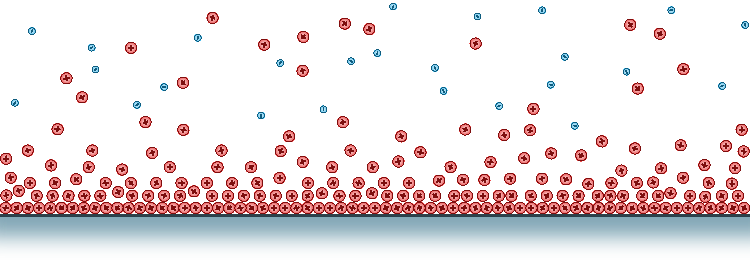
\includegraphics{content/pt1/01-PowerHarvesting/graphics/intro_2_wall}
      \caption{
        \label{fig:doubleLayerBetweenWalls}
        Formation of a double layer along a solid wall.
      }
  \end{figure}
  Consider a double layer that has formed along a perfectly flat surface.
  \Cref{fig:doubleLayerBetweenWalls} illustrates this situation, where the walls are negatively charged and therefore the counter-ions are positively charged.
  Counter-ions, separated from the bulk of the liquid, line the exterior of the wall; but charge separation is not enough to generate electrical power.

  % Harvesting energy
  \begin{figure}
      \centering
      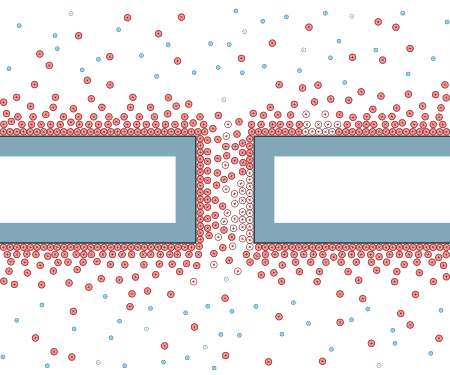
\includegraphics{content/pt1/01-PowerHarvesting/graphics/intro_2_channel_relaxed}
      \caption{
        \label{fig:doubleLayerInChannel_noPressure}
        Double layer formation within a streaming cell that is in a state of equilibrium.
      }
  \end{figure}
  Energy can not be created or destroyed, it must be converted from one form to another.
  In this case, counter-ions are electrostatically bound to the interface and removing them requires work.
  Although the counter-ion density has been increased at the boundary, the charge is not free.
  Migration of charge to the walls ceases once the surface potential has been neutralised.
  Double layer formation takes work to undo and the process stops once the layer is formed.
  Generating electrical energy requires taking some form of power from the fluid, in this case mechanical.
  Liquids pass mechanical power in the form combination a pressure and a flow.
  Harvesting power from liquid will cause a drop in pressure as liquid is pushed through the harvesting mechanism.
  The mechanisms presented here use mechanical power to shift the ionic balance between two bodies of liquid.
  This means separating and isolating negative and positive ions from each other.  
  Figure~\ref{fig:doubleLayerInChannel_noPressure} shows another charged wall, but with the addition of a small channel.
  Notice that the channel contains no co-ions, it is exclusively occupied by counter-ions.
  The ratio of counter-ions to co-ions within the channel is controlled by the width of the channel.
  The narrower the channel, the less likely it is for co-ions to get inside.
  This channel is small enough that the layers overlap one another, repelling co-ions.
  The channel and the two separated bodies of liquid now form an energy harvester.
  Counter-ion rich fluid is transported across the channel by applying a pressure differential.
  As counter-ions exit the channel on the low-pressure side, new ions move to replenish the double layer on the high-pressure side.
  \begin{figure}
      \centering
      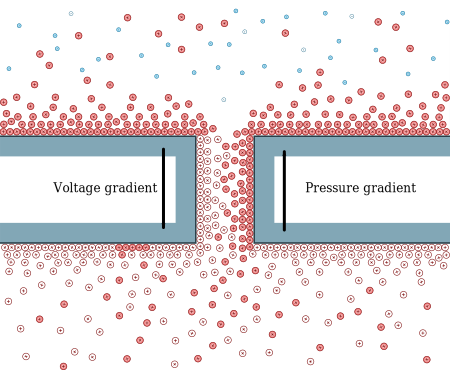
\includegraphics{content/pt1/01-PowerHarvesting/graphics/intro_2_channel}
      \caption{\label{fig:doubleLayerInChannel_withPressure}Double layer formation within a streaming cell that has a pressure differential applied.}
  \end{figure}
  A diagram showing the channel geometry, but with pressure applied and a voltage gradient generated is shown as figure~\ref{fig:doubleLayerInChannel_withPressure}.
  The, including the non-conductive wall, is referred to as a streaming cell.
  Streaming cells are able to continuously separate ions of an electrolyte fluid.
  Electrical potential across a streaming cell increases as those ions are pumped through.
  This only works when the solid surface has charge at its surface, necessary to form the double layer.

  % Channel fabrication and materials
  A channel can be created individually using a range of fabrication methods, such as chemical etching or using narrowly separated parallel plates.
  They can also be formed en-mass by using porous materials such as glass or ceramics, where the pores themselves act as channels.
  Glass has the convenient property that it obtains a negative surface charge when in contact with water.
  This surface charge is caused by the deprotonation of surface silanol groups in glass (SiOH~$\leftrightarrows$~SiO$^{-}+$~H$^{+}$)~\cite{Kirby2004}.
  By immersing a glass channel in an electrolyte solution, double layers of counter-ions (positive ions in this case) line the channel walls.
  This means that glass channels have a high voltage on the low-pressure side and a low voltage on the high-pressure side.

  % Limitations of prevous content
  The concept behind the device is relatively straight-forward, but the physical reality is complex.
  The diagrams presented here are simplified, having perfectly flat walls containing single atom ions carrying a single charge.
  No mention of molecules has been made, which increases the complexity.
  Polar molecules such as water have positive and negative components offset in space.
  Although simplified, this material illustrates the how streaming cells work.
  Next, literature concerning the operation, design and improvements to streaming cell technology is presented and discussed.


\section{Review of Streaming Cell Literature}

  % Initial work of Osterle
  \begin{figure}
    \centering
    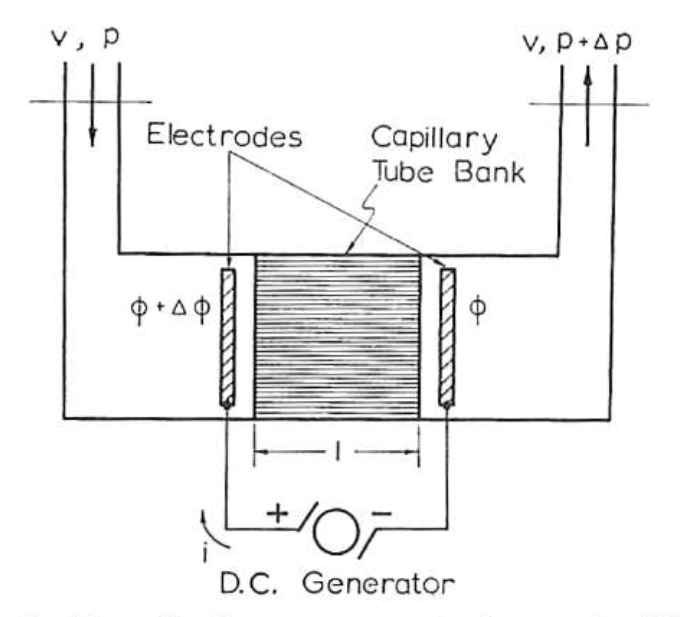
\includegraphics[height=6cm]{content/pt1/Osterle_ElectrokineticCell.png}
    \caption{\label{fig:Osterle_cell}Osterle's electrokinetic pumping cell, reproduced from \cite{Osterle1964}}
  \end{figure}
  In 1964, a paper by Osterle gave an analysis of energy conversion from streaming cells, both for the purpose of pumping or generating electrical power was presented~\cite{Osterle1964}.
  The cell he used consisted of fine capillary tubes stacked together to form a streaming cell.
  A diagram of that cell, in its pumping configuration, is reproduced here as~\cref{fig:Osterle_cell}.
  Importantly, he shows that a streaming cell has the same conversion efficiency whether it is in a pumping mode, where electrical energy is supplied, or in a generating mode, where electrical energy is produced.
  Based on his analysis, Osterle gives an illustrative example of an streaming cell producing electrical energy.
  He states that tube bank having a volume of \SI{100}{\centi\meter\cubed} with \SI{100}{\kilo\pascal} of hydrostatic pressure applied would be capable of producing \SI{0.49}{\watt} of electrical energy.
  This would require \SI{125}{\watt} of pumping power to achieve, giving an energy conversion efficiency of \SI{0.392}{\percent}.

  % Another, paper - the beginning of streaming cells
  Within the space of a year three papers related to properties of fluid flow in fine capillaries, such as those used by Osterle are presented.
  Burgreen and Nakache investigate both the flow when the capillaries are rectangular~\cite{Burgreen1964}, and the efficiency of such capillaries when used to generate electrical power or to pump~\cite{Burgreen1965}. 
  Their work develops mathematics behing rectangular streaming cells and shows fine glass capiliaries are equally efficient when used to generate electrical power or to induce liquid pumping.
  Rice and Witehead make an analysis of fluid flow profiles that consider the effect of double layer interactions~\cite{Rice1965}.
  They show how the double layer affects the level to which liquid can permeate a material populated with cavites.
  Together these three papers mark the beginning of research into streaming cells.

  % Renewed interest and dimensions
  There appears to be little published research into streaming cells until 2003, when a surge of papers related to optimal dimensions of streaming cells appear.
  An analysis relating energy conversion efficiency to the length of a streaming cell channel indicated that short cells are the most efficient~\cite{Yang2003}.
  However, more recent work by Chang and Yang shows a decrease in conversion efficiency at maximum power when the channel length is low~\cite{Chang2009}.
  This work suggests there is an optimum channel length, which is also dependant on the fluid conductivity.
  Investigation into the relationship between the Debye length of the double layer and streaming cell conversion efficiency found that a channel is most efficient when its height is twice that of the Debye length~\cite{Daiguji2004}
  This corresponds to the point at which double layers formed within a cell begin to overlap with one another.  

  In 2005 a seminal paper by van der Heyden et al.\ reported on streaming cell measurements made in a single microchannel \SI{70}{\micro\meter} in height~\cite{VanderHeyden2005}.
  Many valuable contributions were detailed in this paper, namely:
  \begin{enumerate}
    \item Confirmed that reversing the polarity of surface potential reverses the direction of the streaming current.
    \item Found that the maximum conversion efficiency corresponded to channels where double layers begin to overlap. This confirms the relationship put forward the previous year by Daiguji et al.\
    \item Show that boundary conditions involving constant surface potentials, used up to this point to model streaming, are inaccurate.
    \item Predict a maximum energy conversion efficiency of $\sim$\SI{6}{\percent} for potassium chloride solutions of \SI{1e-5}{\mole} in silica channels of height \SI{145}{\nano\meter}.
  \end{enumerate}
  Subsequent research by the same authors reported that energy conversion efficiency is maximised at low salt concentrations~\cite{VanderHeyden2006}. 
  In which they predicted a \SI{12}{\percent} efficiency for streaming cells using electrolyte solutions of lithium.
  Around the same time, Daiguji et al.\ publish work suggesting that in order to increase cell efficiency one may either reduce the channel height or decrease the ionic concentration of the working fluid~\cite{Daiguji2006}.
  This supports the work of van der Heyden et al.\ with respect to efficiency gains with the working fluids having low ionic concentrations.

  % Stern conductance
  In 2007, van der Heyden et al.\ publish a measured energy conversion of \SI{3.2}{\percent}~\cite{Heyden2007}.
  They suggest that the conversion efficiency of a channel is limited by a property termed `Stern conductance'.
  The concept of stern conductance is that the stern layer (see \cref{fig:doubleLayer_anatomy}) itself provides a pathway for electrical conduction.
  This conduction turns the surface of the glass into an electrically conductive surface causing the cell to partially self-discharge.
  Stern conductance is often referred simply as `surface conductance'.
  Davidson and Xuan published a mathematical model shortly after confirming the role of Stern conductance on streaming cells, in particular those with low ionic strength~\cite{Davidson2008}.
  They suggest that this is the reason for poor measured efficiencies in light of the much higher predicted values.

  % Hydrodynamic slip
  \begin{figure}
    \centering
    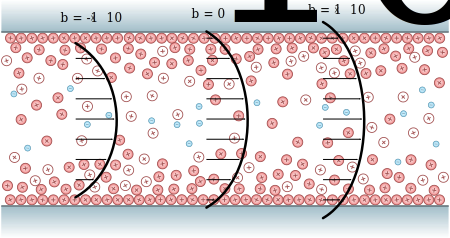
\includegraphics[height=6cm]{content/pt1/graphics/HydrodynamicSlip}
    \caption{\label{fig:HydrodynamicSlip}Illustration of hydrodynamic slip inside a channel cavity, where $b$ is the slip length. Arrows indicate flow velocity in each of the three situations.}
  \end{figure}
  Most recently, the concept of hydrodynamic slip has been applied to streaming cells as a way of increasing conversion efficiency.
  Estimates using mathematical models predicted conversion efficiencies between \SI{30}{\percent} and \SI{70}{\percent}~\cite{Pennathur2007, Davidson2008a, Ren2008}.
  Hydrodynamic slip refers to the ability of a fluid to `slip' relative to a boundary/interface.
  Slip is advantageous to streaming cells because ions in the Stern layer to move against the solid's surface.
  The length refers to an imaginary distance into the solid wall where the traditional `no-slip' boundary condition would occur (refer to~\cref{fig:HydrodynamicSlip}).
  A `no-slip' boundary condition dictates that fluid at the boundary of a solid must have zero velocity.
  This condition, along with viscosity, is responsible for the parabolic flow profile a fluid takes as it moves through pipes.
  An issue surrounding slip was illustrated by Eijkel who showed that a channel's zeta potential and its slip length are linked~\cite{Eijkel2007}.
  The general problem with slip based mechanisms is that a high zeta potential is optimal for double layer formation, however it also promotes wetting.
  Wetting and hydrodynamic slip are related to each other by the strength of attraction between a liquid and a solid.
  To explain, the terms hydrophobic and hydrophilic are used to describe surfaces that repel and attract water. 
  A hydrophobic surface has a low tendency to support water, i.e., water will bead and roll off a hydrophobic surface.
  Conversely, a hydrophilic surface is one that water \emph{is} attracted to, causing a droplet to spread and stick to the surface.
  Hydrodynamic slip occurs when a channel's walls are hydrophobic, allowing water at the interface to slip along the boundary of the solid.
  High zeta potentials attract water to the solids surface due to electrostatic attraction.
  Eijkel's publication illustrates that the zeta potential and hydrodynamic slip are related to one another. 
  In order to improve the situation in steaming cells a surface should be both non-wetting and hold a high surface charge.
  Conservative estimates place an efficiency of \SI{40}{\percent} on cells having slip lengths tens of nanometers long, obtainable using carbon nanotubes, using solutions having low salt concentration.


  %Research around streaming cell energy conversion headed in a new direction after an article written by Pennathur et al.\ in 2007 detailed a mathematical model predicting the effects of hydrodynamic slip~\cite{Pennathur2007}.
  %It proposed efficiency figures as high as \SI{30}{\percent} for a slip length of \SI{6.5}{\nano\meter} in cylindrical tubes \SI{100}{\nano\meter} in diameter.


  %Eijkel, in a follow-up publication to that of Pennathur's, discusses the relationship between zeta potential and slip length~\cite{Eijkel2007}.

  %\begin{figure}
    %\centering
    %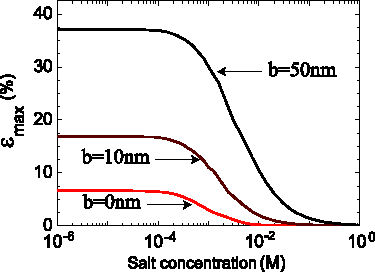
\includegraphics[height=6cm]{content/pt1/graphics/SteinSlipEnchancedChannelEfficiency}
    %\caption{\label{fig:Stein_Slip_Prediction}Plot of predicted efficiency versus salt concentration for various for slip lengths of 0, 10 and \SI{50}{\nano\meter}, taken from~\cite{Ren2008}.}
  %\end{figure}

  %That same year, two papers modelling the effects of hydrodynamic slippage were published.
  %The first, by Davidson and Xuan, gives a mathematical prediction of the effects of hydrodynamic slippage at the interface surface~\cite{Davidson2008a}.
  %They predict that when taking slip at the solid-fluid boundary into consideration that conversion efficiencies as high as \SI{30}{\percent} should be obtainable.

  %The second, by Ren and Stein, predict conversion efficiencies as high as \SI{70}{\percent} based on the slip lengths recently observed with carbon nanotubes~\cite{Ren2008}.
  %They provide a more conservative prediction of \SI{40}{\percent} for slip lengths in the tens of nanometers region and low salt concentration.

  % Summary
  Theoretical predictions of the efficiency of standard micro/nano-fluidic channels are 2\% for pure water and 7\% for sodium chloride.~\cite{VanderHeyden2006}
  However, measured conversion efficiencies as reported thus far are:
  \begin{itemize}
    \item ``far less than \SI{1}{\percent}'' forcing potassium chloride through a porous glass plug having pores in the range \SI{1}--\SI{1.6}{\micro\meter}~\cite{Olthuis2005}.
    \item 0.01\% by forcing water through porous glass with pore sizes from 10\thinspace--\SI{16}{\micro\metre}.~\cite{Yang2003}
    \item 0.8\% by forcing pure water through a ceramic rod populated with \SI{6}{\micro\metre} pores.~\cite{Yang2004}
    \item 3\% by forcing a sodium chloride solution through a \SI{75}{\nano\metre} by \SI{50}{\micro\metre} silica channel.~\cite{Heyden2007}
    \item 0.77\% by forcing a sodium chloride solution through a \SI{200}{\nano\metre} pore in an alumina membrane.~\cite{Lu2006}
    \item 5\% by forcing a sodium chloride solution through a \SI{0.5}{\nano\metre} cylindrical pore in polyethylene terephalate foil.~\cite{Xie2008}
  \end{itemize}
  It is clear from the literature that there is significant progress to be made with respect to increasing the conversion efficiency of streaming cells.
  Techniques to induce hydrodynamic slip at the fluid-solid interface are predicted to increase this efficiency to 30-40\%~\cite{Davidson2008a, Ren2008}, but progress in this area is dictated by advancements in materials science.
  Experimental results utilising slip enhanced channels have not yet been reported in the literature.
  Surface enhanced channels will not be investigated due to manufacturing difficulty, cost, and the level of scientific development required to make progress.

  %In 2012, Cherng Hon et al.\ presented a novel method of producing electrokinetic power from steaming cells using salinity gradients~\cite{CherngHon2012}.
  %In this work the authors describe a system where flow through a conventional streaming cell is brought about by forward osmosis.
  %This allows the authors to generate electrical energy from streaming cells without mechanical pumping.
  %The application has limited use, but it highlights novel uses for streaming cells as a means of electrical generation.

  %Most recently, in 2014, Jiao et al.\ presented results showing that surface treatment of porous glass can increase conversion efficiency~\cite{Jiao2014}.
  %They show that ultrasonically pre-treating glass and subsequently applying Sodium Dodecyl Sulphate to the surface gave a relative increase of \SI{27.3}{\percent} in power density.
  %Unfortunately, they do not state the absolute efficiency of their channels in either case.

  %Theoretical predictions of the efficiency of standard micro/nano-fluidic channels are 2\% for pure water and 7\% for sodium chloride.~\cite{VanderHeyden2006}
  %Experimental results show conversion efficiencies in the range of:
  %These results indicate that small channels using solutions containing salt are more efficient.
  %According to \cite{Daiguji2004}, the efficiency is maximised when the channel height twice that of the Debye length.
  %Additionally, ~\cite{VanderHeyden2006} states that the maximum efficiency is found when the salt concentration is low.

  In summary, the finding that maximum conversion efficiency occurs at low ionic concentration supports the use of tap-water as a working fluid.
  The use of glass as a substrate appears to be a suitable choice, which is both cost effective and a convenient material.
  The dimensions of cells found in the literature suggest fabricate trial cells is feasible with the equipment available.
  It appears that a conversion efficiency of \SI{0.01}{\percent} should be achievable using a porous glass plug.

